\chapter{SVM: Support Vector Machines}\label{chap:svm}

Le SVM sono modelli di machine learning supervisionato che possono essere utilizzati sia per problemi di classificazione che di regressione.  L'idea alla base delle SVM è trovare un iperpiano che separi i dati di diverse classi con il massimo margine possibile: sono quindi una delle soluzioni più eleganti e semplici da visualizzare per quando riguarda la classificazione. L'iperpiano scelto non solo separa le classi, ma lo fa in modo tale da \textbf{massimizzare la distanza tra l'iperpiano e i punti} più vicini di ciascuna classe, noti come vettori di supporto. 

\section{Iperpiani di separazione}
Dati i vettori $x_i$ e $x_j$, un modo di definirne la similarità è il prodotto scalare tra i due\footnote{In generale, il prodotto scalare tra due vettori $a$ e $b$ è definito come $a^T b = \|a\| \, \|b\| \cos \theta$.} :
\[
\langle x_i, x_j \rangle = x_i^T x_j = \|x_i\| \, \|x_j\| \cos\theta
\]
dove $\|x_i\|$ e $\|x_j\|$ sono le norme dei vettori $x_i$ e $x_j$, e $\theta$ è l'angolo tra i due vettori. Da questo si evince che la similarità tra i due vettori è massima quando sono paralleli (ovvero quando $\theta = 0$), e minima quando sono ortogonali (ovvero quando $\theta = 90^\circ$).

Il valore di questo prodotto dipende dalla norma\footnote{La norma di un vettore è una misura della sua lunghezza o grandezza, come il modulo di un vettore in uno spazio euclideo.} dei due vettori. Questo permette di definire un iperpiano di separazione come l'insieme dei punti $x$ che soddisfano l'equazione:
\[
\langle w, x \rangle + b = 0
\]
dove $w$ è un vettore normale all'iperpiano e $b$ è l'intercetta.

\subsection{Funzione di decisione lineare}
L'idea principale dietro a diversi algoritmi di classificazione è quello di rappresentare i dati in uno spazio $\mathbb{R}^d$, dove $d$ è il numero di features del piano, e trovare quel \emph{decision boundary} grazie al quale l'algoritmo è capace di separare le diverse classi. Nel caso di una classificazione binaria si separa lo spazio in due regioni corrispondenti alla classe positiva e negativa e si cerca quell'iperpiano che separa le due regioni. Sia $x \in \mathbb{R}^d$ un esempio nello spazio dei dati, consideriamo la funzione:
\[
f: \mathbb{R}^d \rightarrow \mathbb{R}, \quad f(x) := \langle w, x \rangle + b
\]
dove $w \in \mathbb{R}^d$ e $b \in \mathbb{R}$ sono rispettivamente il vettore dei pesi e il bias. In questo modo, un iperpiano può essere definito come il \textbf{separatore} lineare delle due classi, ovvero:
\begin{equation}
	\{ x \in \mathbb{R}^d : f(x) = 0 \}
	\label{eq:svm_hyperplane}
\end{equation}

\begin{figure}[htbp]
    \centering
    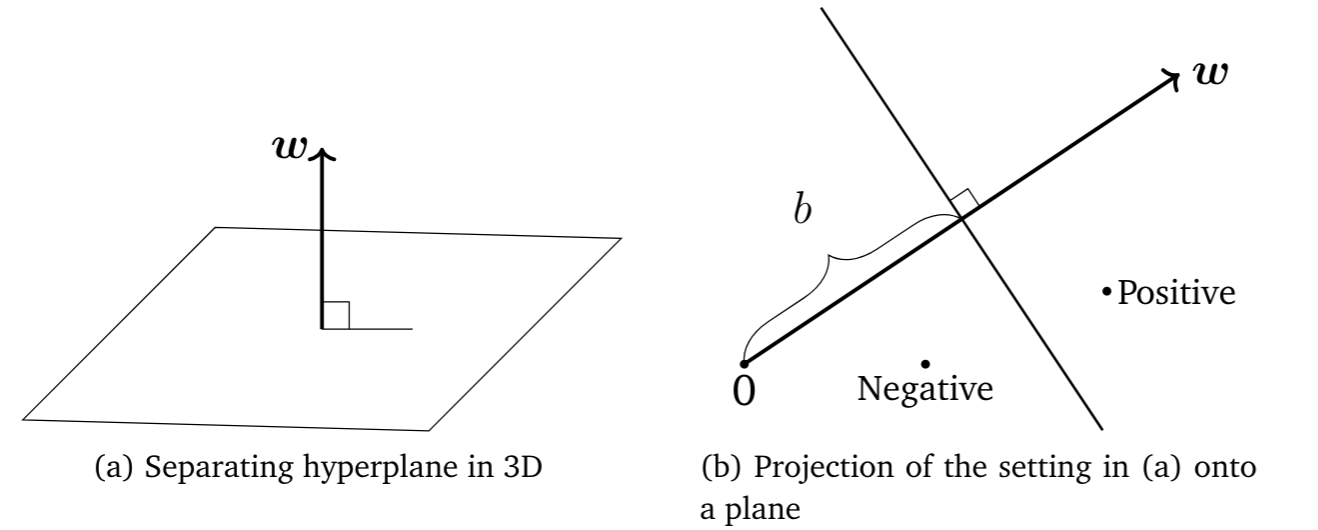
\includegraphics[width=\textwidth]{images/svm_hyperplane.png}
    \caption{Esempio di iperpiano come frontiera di decisione: il vettore $w$ è normale all'iperpiano e ne determina l'orientamento, mentre il termine $b$ ne stabilisce la posizione rispetto all'origine, separando i punti delle due classi sul lato positivo e su quello negativo.}
    \label{fig:svm_hyperplane}
\end{figure}

\subsection{Interpretazione geometrica}
Come si vede in figura \ref{fig:svm_hyperplane}, il vettore $w$ è normale\footnote{Un vettore è normale a un iperpiano se è perpendicolare a ogni vettore che giace sull'iperpiano.} all'iperpiano e ne determina l'orientamento, mentre il termine $b$ ne stabilisce la posizione rispetto all'origine, separando i punti delle due classi sul lato positivo e su quello negativo. Questo è anche possibile dimostrarlo prendendo in considerazione due esempi $x_a, x_b$ giacenti sull'iperpiano:
\begin{align*}
    &f(x_a) = f(x_b) \\
    \Rightarrow \quad
    &f(x_a) - f(x_b) = 0 \\
    \Rightarrow \quad
    &(\langle w, x_a \rangle + b) - (\langle w, x_b \rangle + b) = 0 \\
    \Rightarrow \quad
    &\langle w, x_a \rangle - \langle w, x_b \rangle = 0 
    &(\text{poiché } b-b=0) \\
    \Rightarrow \quad
    &\langle w, x_a - x_b \rangle = 0 
    &(\text{per linearità del prodotto scalare})
\end{align*}

Utilizzando l'equazione dell'iperpiano \eqref{eq:svm_hyperplane}, possiamo, per un certo esempio $x$ capire se si tratta di una classe positiva o negativa a seconda della regione in cui si trova rispetto all'iperpiano:
\[
y = 
\begin{cases}
	+1 & \text{se } f(x) \geq 0 \\
	-1 & \text{se } f(x) < 0
\end{cases}
\]
dove $y$ è l'etichetta di classe associata all'esempio $x$ e $f(x)$ è l'equazione dell'iperpiano. Questo si può rappresentare tramite la quantità chiamata \textbf{margine funzionale}:
\begin{equation}
\gamma(x) = y \, (\langle w, x \rangle + b).
\label{eq:svm_functional_margin}
\end{equation}
Un esempio è correttamente classificato se
\[
y \, (\langle w, x \rangle + b) \ge 0.
\]

\section{Primal SVM}
Questa formulazione delle SVM ha l'obiettivo di trovare quell'iperpiano che massimizza il margine tra le due classi. Ipotizziamo un dataset $\{(x_1, y_1), \ldots, (x_n, y_n)\}$ linearmente separabile, dove $x_i \in \mathbb{R}^d$ sono gli esempi e $y_i \in \{-1, +1\}$ sono le etichette di classe. Esistono infiniti iperpiani che possono separare le due classi, ma possiamo dire che un iperpiano è migliore di un altro se performa meglio sui dati di test. Formuliamo quindi un vero e proprio \textbf{problema di ottimizzazione}, cui risoluzione ci offrirà i valori ottimali di $w$ e $b$.

\subsection{Concetto di margine}\label{sec:svm_margin}
L’idea chiave delle SVM (nel caso linearmente separabile) è scegliere, tra i molti iperpiani separatori possibili, quello che \emph{massimizza il margine}, cioè la distanza tra l’iperpiano di decisione e gli esempi più vicini (i futuri \emph{support vectors}). Per formalizzare questa intuizione dobbiamo però chiarire un punto tecnico: \emph{a quale scala} misuriamo questa distanza?

\paragraph{Invarianza di scala.}
L’iperpiano
\[
\langle w, x\rangle + b = 0
\]
non cambia se moltiplichiamo \emph{entrambi} i parametri per una costante positiva $\alpha>0$:
\[
\langle \alpha w, x\rangle + \alpha b = 0
\quad\Longleftrightarrow\quad
\langle w, x\rangle + b = 0.
\]
Quindi, se non fissiamo una convenzione di scala, quantità come $\langle w,x\rangle+b$ (e derivate) possono essere rese arbitrariamente grandi o piccole senza modificare la frontiera di decisione. Per evitare ambiguità, nella derivazione geometrica fissiamo la scala \emph{normalizzando} il vettore normale all’iperpiano, cioè imponendo $\|w\|=1$ (norma euclidea).

\paragraph{Distanza punto-iperpiano (proiezione ortogonale).}
Consideriamo un esempio $x_a$ e la sua proiezione ortogonale $x'_a$ sull’iperpiano (Figura~\ref{fig:svm_margin}). Poiché $w$ è normale all’iperpiano, il segmento che unisce $x'_a$ a $x_a$ è parallelo a $w$. Introduciamo allora una distanza $r>0$ tale che
\[
x_a = x'_a + r\,\frac{w}{\|w\|}.
\]
Se imponiamo $\|w\|=1$, il termine $\frac{w}{\|w\|}$ è un versore e $r$ coincide con la distanza euclidea tra $x_a$ e l’iperpiano.

Poiché $x'_a$ giace sull’iperpiano, vale $\langle w,x'_a\rangle+b=0$. Sostituendo $x'_a = x_a - r\frac{w}{\|w\|}$ otteniamo
\begin{align*}
\Big\langle w, x_a - r\frac{w}{\|w\|}\Big\rangle + b 
&= 0 
\\
\Longleftrightarrow \quad
\langle w, x_a\rangle 
- r \left\langle w, \frac{w}{\|w\|} \right\rangle 
+ b 
&= 0 
\\
\Longleftrightarrow \quad
\langle w, x_a\rangle 
- r \frac{\langle w,w\rangle}{\|w\|} 
+ b 
&= 0 
\\
\Longleftrightarrow \quad
\langle w, x_a\rangle 
- r \frac{\|w\|^2}{\|w\|} 
+ b 
&= 0 
\\
\Longleftrightarrow \quad
\langle w, x_a\rangle 
- r \|w\| 
+ b 
&= 0 
\\
\Longleftrightarrow \quad
\langle w, x_a\rangle + b 
&= r\,\|w\| 
\end{align*}

Con la normalizzazione $\|w\|=1$ segue semplicemente
\[
r = \langle w,x_a\rangle + b.
\]
In altre parole, quando $\|w\|=1$, il valore della funzione affine $f(x)=\langle w,x\rangle+b$ (sul lato positivo) misura direttamente la distanza geometrica dall’iperpiano.

\begin{figure}[htbp]
    \centering
    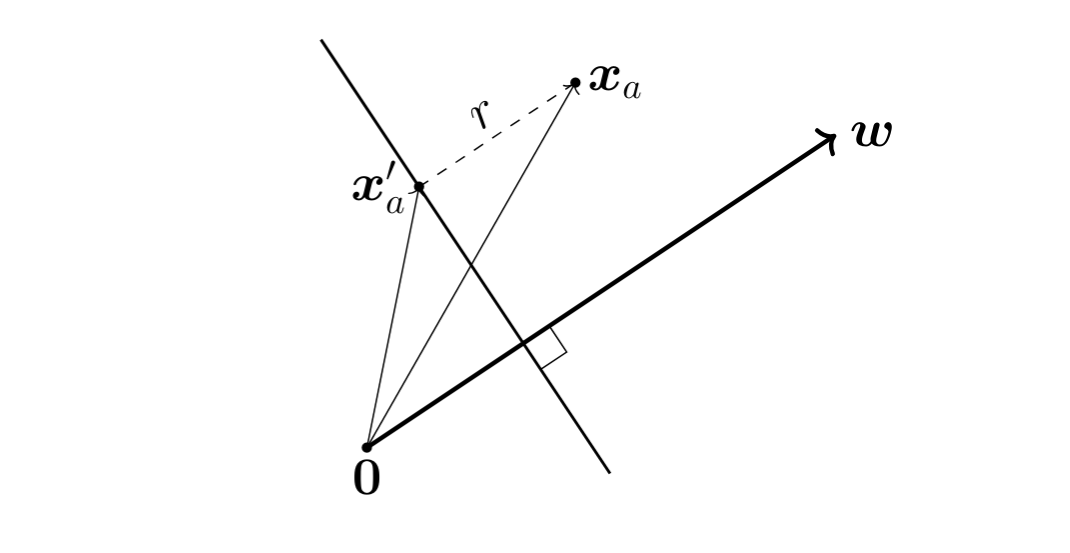
\includegraphics[width=0.8\textwidth]{images/svm_margin_distance.png}
    \caption{Distanza $r$ tra un punto $x_a$ e la sua proiezione ortogonale $x'_a$ sull'iperpiano di separazione.}
    \label{fig:svm_margin}
\end{figure}

\paragraph{Il margine come vincolo sui dati.}
Vogliamo che \emph{tutti} gli esempi siano correttamente classificati e si trovino almeno a distanza $r$ dall’iperpiano, sul lato coerente con l’etichetta. Questo si esprime in un’unica disuguaglianza:
\[
y_n\big(\langle w,x_n\rangle + b\big) \ge r,
\qquad n=1,\dots,N,
\]
dove $r>0$ è il margine (distanza del punto più vicino). A questo punto l’obiettivo è massimizzare $r$, mantenendo la normalizzazione $\|w\|=1$. Otteniamo quindi il problema di ottimizzazione (hard margin, vista geometrica):
\[
\max_{w,b,r}\; r
\quad
\text{soggetto a}\quad
y_n(\langle w,x_n\rangle + b)\ge r,\;\; \|w\|=1,\;\; r>0.
\]
Questo formalizza esattamente l’idea: scegliere l’iperpiano che “separa di più” le due classi, cioè quello che lascia il cuscinetto (margin) più ampio attorno alla frontiera di decisione.

\subsection{Derivazione tradizionale}\label{sec:svm_traditional_derivation}
Un modo equivalente per arrivare alla formulazione \emph{primal} consiste nel fissare la scala in maniera diversa: invece di imporre $\|w\|=1$, si scala $(w,b)$ in modo che il (o uno dei) punti più vicini all’iperpiano soddisfi
\[
\langle w, x_a\rangle + b = 1,
\]
cioè si pone il margine “a unità” sulle ipersuperfici parallele $\langle w,x\rangle+b=\pm 1$. Con questa convenzione si ricava che la distanza geometrica del punto più vicino (il margine) risulta proporzionale a $\tfrac{1}{\|w\|}$, quindi massimizzare il margine equivale a minimizzare la norma di $w$.

In questa scala, la corretta classificazione con margine unitario si scrive come
\[
y_n(\langle w,x_n\rangle + b)\ge 1,\qquad n=1,\dots,N.
\]
Il problema di ottimizzazione finale (hard margin SVM) diventa quindi
\[
\min_{w,b}\; \frac{1}{2}\|w\|^2
\quad
\text{soggetto a}\quad
y_n(\langle w,x_n\rangle + b)\ge 1,\;\; n=1,\dots,N,
\]
dove il termine $\tfrac12\|w\|^2$ è scelto per comodità analitica (derivate più “pulite”) senza cambiare il minimizzatore.

\medskip
\noindent
\textit{\textbf{Nota}: si può trovare un approfondimento sulla dimostrazione di questa equivalenza nella sezione \ref{sec:teorema_margine_1} del capitolo \ref{chap:approfondimenti_teorici}.}

\section{Soft Margin SVM}
Nel caso di dati non linearmente separabili, potremmo desiderare di permettere ad alcuni esempi di cadere all'interno dell'area del margine, o addirittura di finire dalla parte sbagliata dell'iperpiano. Il modello che permette alcuni errori di classificazzione, è detto \textbf{soft margin SVM}. Introduciamo una variabile, detta \textbf{variabile di slack}, indicata con $\xi_n$. Sottrarre questo termine, ci permetterà di rilassare i \textit{contrains} relativi alla classificazione, consentendo errori.

$$
\begin{aligned}
	&\min_{w,b,\xi} && \frac{1}{2}\|w\|^{2} + C \sum_{n=1}^{N} \xi_n \\
	&\text{rispetto a} && y_n \big( \langle w, x_n \rangle + b \big) \ge 1 - \xi_n, \\
	& && \xi_n \ge 0
\end{aligned}
$$

La variabile di slack dovrà essere non-negativa. Il parametro $C>0$ nella funzione obiettivo gestisce il tradeoff tra la dimensione del margine e la dimensione complessiva di rilassamento. È detto \textbf{parametro di regolarizzazione}. Indichiamo invece con il nome \textbf{regolarizzatore} il termine $\|w\|^2$, questo controlla la larghezza del margine. 

\begin{itemize}
	\item $C$ \textbf{grande}: penalizzi molto le $\xi_n$. Il modello cercherà di commettere pochissimi errori, anche se questo porta ad avere un margine più stretto, rischiando \textbf{overfitting}.
	\item $C$ \textbf{piccolo}: gli errori costano poco, accettando più violazioni, in cambio con un margine più grande, ottenendo un modello più regolare.
\end{itemize}


\subsection{Soft Margin SVM e Loss function}
Cambiamo il nostro approccio alle SVM, seguendo il \textbf{principio di minimizzazione del rischio empirico}\footnote{Nella teoria dell'apprendimento statistico, la minimizzazione del rischio empirico (in inglese empirical risk minimization, da cui la sigla ERM) è un principio che definisce una famiglia di algoritmi di apprendimento e viene utilizzato per fornire limiti teorici alle loro prestazioni.
L'idea centrale è che non è possibile sapere esattamente quanto bene funzionerà un algoritmo nella pratica (il "rischio vero") perché è ignota la vera distribuzione dei dati su cui lavorerà l'algoritmo, ma è invece possibile misurarne le prestazioni su un insieme di dati di addestramento noto (il rischio "empirico").}. 
Nel modello SVM, scegliamo come classe di ipotesi\footnote{insieme di tutti i modelli possibili che consideriamo} gli iperpiani, ossia funzioni del tipo

$$f(x) = \langle w, x \rangle + b$$

dove il margine, coincide con il termine di regolarizzazione. Affrontiamo adesso l'argomento relativo alla loss function, che dovrà essere mirata al task principale del modello, ossia classificazione binaria. 

\paragraph{Zero-One Loss.}

La \textbf{zero-one loss} misura se una predizione è corretta oppure no.
L'obiettivo sarebbe minimizzare il numero di esempi per cui la classe
predetta $\hat{y}_n = \mathrm{sign}(f(x_n))$ non coincide con
l'etichetta reale $y_n$.

Nel caso di classificazione binaria con $y_n \in \{-1,+1\}$,
possiamo esprimere questa loss tramite la funzione indicatrice come

\[
\mathbf{1}\big(y_n f(x_n) \le 0\big).
\]

Infatti:
\begin{itemize}
    \item se $y_n f(x_n) > 0$, la predizione è corretta;
    \item se $y_n f(x_n) \le 0$, la predizione è errata.
\end{itemize}

Il rischio empirico associato diventa quindi

\[
\sum_{n=1}^{N}
\mathbf{1}\big(y_n f(x_n) \le 0\big).
\]

Tuttavia, questa funzione è non continua e non convessa.
Minimizzarla porta a un problema di ottimizzazione combinatorio,
generalmente difficile da risolvere in modo efficiente.

\paragraph{Hinge Loss.}

La \textbf{hinge loss} è una funzione di perdita convessa che penalizza non solo le classificazioni errate, ma anche quelle corrette che si trovano troppo vicine all'iperpiano di separazione. L'idea è sostituire la zero-one loss con una funzione continua e convessa, più semplice da ottimizzare, che favorisca un margine ampio.

Consideriamo l'errore tra l'output del predittore $f(x_n)$ e l'etichetta $y_n$. Ci aspettiamo loss nulla quando la predizione è corretta e si trova al di fuori del margine (cioè quando il vincolo di margine è soddisfatto). Una predizione corretta ma all'interno del margine viene comunque penalizzata, mentre una predizione errata riceve una penalizzazione maggiore.

La hinge loss è definita come
\[
L(t) = \max\{0,\, 1-t\},
\qquad
t = y_n f(x_n) = y_n(\langle w, x_n \rangle + b).
\]

Equivalentemente, può essere scritta come funzione a tratti:
\[
L(t)=
\begin{cases}
0 & \text{se } t \ge 1,\\
1-t & \text{se } t < 1.
\end{cases}
\]

\section{Dual SVM}\label{sec:dual_svm}

La formulazione duale delle SVM si ottiene applicando i moltiplicatori
di Lagrange alla formulazione primale. Invece di ottimizzare
direttamente sui parametri $w$ e $b$, il problema viene riscritto
in termini dei moltiplicatori $\alpha_n$, uno per ogni esempio
del dataset.

Un risultato fondamentale è che il vettore dei pesi ottimale può
essere espresso come combinazione lineare dei dati di training:

\[
w = \sum_{n=1}^{N} \alpha_n y_n x_n.
\]

Nel problema duale, la funzione obiettivo dipende esclusivamente
dai prodotti scalari tra coppie di esempi:

\[
\langle x_i, x_j \rangle.
\]

L'ottimizzazione avviene quindi rispetto agli $\alpha_n$,
soggetti ai vincoli

\[
\sum_{n=1}^{N} \alpha_n y_n = 0,
\qquad
0 \le \alpha_n \le C.
\]

Questa formulazione ha due conseguenze importanti:
\begin{itemize}
    \item la complessità dipende dal numero di esempi $N$,
    non dal numero di feature $D$;
    \item poiché compaiono solo prodotti scalari tra dati,
    è possibile sostituire $\langle x_i, x_j \rangle$
    con una funzione kernel $K(x_i, x_j)$.
\end{itemize}

Questa osservazione è alla base del \textbf{kernel trick}:
lavorare implicitamente in uno spazio delle feature di dimensione
maggiore senza doverlo costruire esplicitamente.

\bigskip
\noindent
\textit{\textbf{Nota}: questa parte è stata scritta solo per riuscire a capire meglio il kernel trick. Un approfondimento completo può essere trovato nella sezione \ref{sec:dual_svm_approfondimento} del capitolo \ref{chap:approfondimenti_teorici}.}

\section{Kernel Trick}

La formulazione Dual SVM è molto potente, in quanto permette l'uso di quello che è noto in letteratura come "\textbf{kernel trick}". Questo torna utile quando i dati non sono linearmente separabili nello spazio originale.

\begin{figure}[tbph]
	\centering
	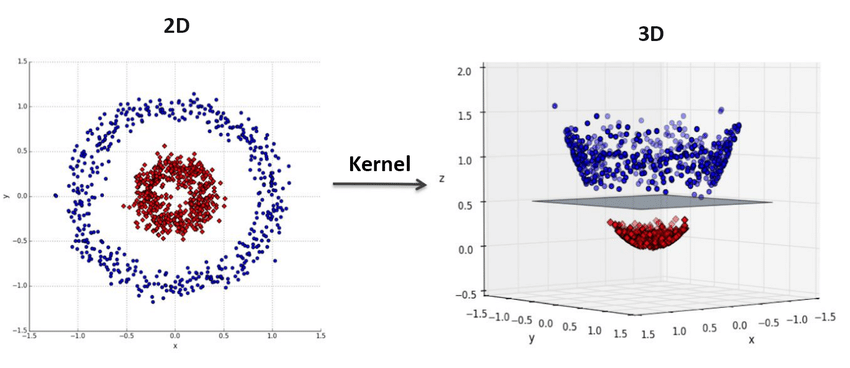
\includegraphics[width=0.75\linewidth]{images/non_linear_SVM}
	\caption{Applicazione di kernel su dati non linearmente separabili. Aumentando di una dimensione, i dati diventano separabili da un iperpiano.}
	\label{fig:nonlinearsvm}
\end{figure}

\subsection{Trasformare i dati}
il nostro desiderio, è quello di lavorare nei dati su uno spazio con più dimensioni rispetto all'originale. Una trasformazione esplicita del dataset $x \to \phi(x)$ in uno spazio più grande, presenta i seguenti rischi:

\begin{itemize}
	\item Vettori molto lunghi a causa delle troppe features ottenute
	\item Costi in termini di calcoli e memoria molto alti
\end{itemize}

\subsection{Il \textit{Kernel Trick}}
Ritorniamo sui nostri passi. La funzione di decisione di un SVM è
$$
\min_{\alpha} \quad
\frac{1}{2} \sum_{i=1}^{N} \sum_{j=1}^{N}
y_i y_j \alpha_i \alpha_j \langle x_i, x_j \rangle
- \sum_{i=1}^{N} \alpha_i 
$$

La formulazione in questione, valuta esclusivamente il prodotto scalare delle coppie di campioni $\langle x_i, x_j\rangle$, che ricordiamo essere indice di somiglianza tra i due campioni valutati. Detto ciò, l'idea è quella di \textbf{sostituire il prodotto scalare con un kernel}, ossia una funzione $K(x, z)$. Questa, matematicamente, si comporta come un prodotto scalare in uno spazio delle features più grande.

$$K(x,z) = \langle \phi(x), \phi(z)\rangle$$

Possiamo quindi evitare il calcolo esplicito di $\phi(x)$, e lavorare sostituendo il prodotto scalare con il kernel più opportuno.

$$
\min_{\alpha} \quad
\frac{1}{2} \sum_{i=1}^{N} \sum_{j=1}^{N}
y_i y_j \alpha_i \alpha_j K(x_i,x_j)
- \sum_{i=1}^{N} \alpha_i 
$$

Ottenendo lo stesso risultato. 

\paragraph{Esempio di applicazione con kernel polinomiale di grado 2}

Immaginiamo di avere due vettori, $x = (x_1, x_2)$ e $z = (z_1, z_2)$.
Supponiamo di mappare $\phi(x)$ e $\phi(z)$, ottenendo
$$\phi(x) =
(
x_1^2,
\sqrt{2}x_1 x_2,
x_2^2,
\sqrt{2}x_1,
\sqrt{2}x_2,
1
) \qquad \phi(z) =
(
z_1^2,
\sqrt{2}z_1 z_2,
z_2^2,
\sqrt{2}z_1,
\sqrt{2}z_2,
1
)$$

\noindent
Il prodotto scalare diventa

$$\langle \phi(x), \phi(z)\rangle = x_1^2 z_1^2 + 2x_1 x_2 z_1 z_2 + x_2^2 z_2^2 + 2x_1 z_1 + 2x_2 z_2 + 1$$

\noindent
Ma lo stesso risultato è ottenibile applicando un kernel polinomiale di grado 2, ossia

$$K(x,z) = (\langle x,z\rangle + 1)^2 = (x_1 z_1 + x_2 z_2 + 1)^2 = x_1^2 z_1^2 + 2x_1 x_2 z_1 z_2 + x_2^2 z_2^2 + 2x_1 z_1 + 2x_2 z_2 + 1$$

Il risultato è il seguente: riusciamo a lavorare su spazi di features molto alti, ma senza mai costruirli. 

\section*{Riferimenti}
Il materiale di questo capitolo è stato tratto da:
\begin{itemize}
	\item Materiale visto a lezione.
	\item Parti del capitolo 12 di \cite{Deisenroth2020MML}.
\end{itemize}
